% !TeX program = PdfLaTeX
% !TeX root = ../Main.tex

\chapter{Results and analysis}
\label{ch3}

In this chapter is presented a case study performed on a regional turboprop of 130 pax, concerning aerodynamic characteristics, high lift devices and ground effect both on wing lift curve and on downwash angle.

\begin{figure}[H]
	\centering
	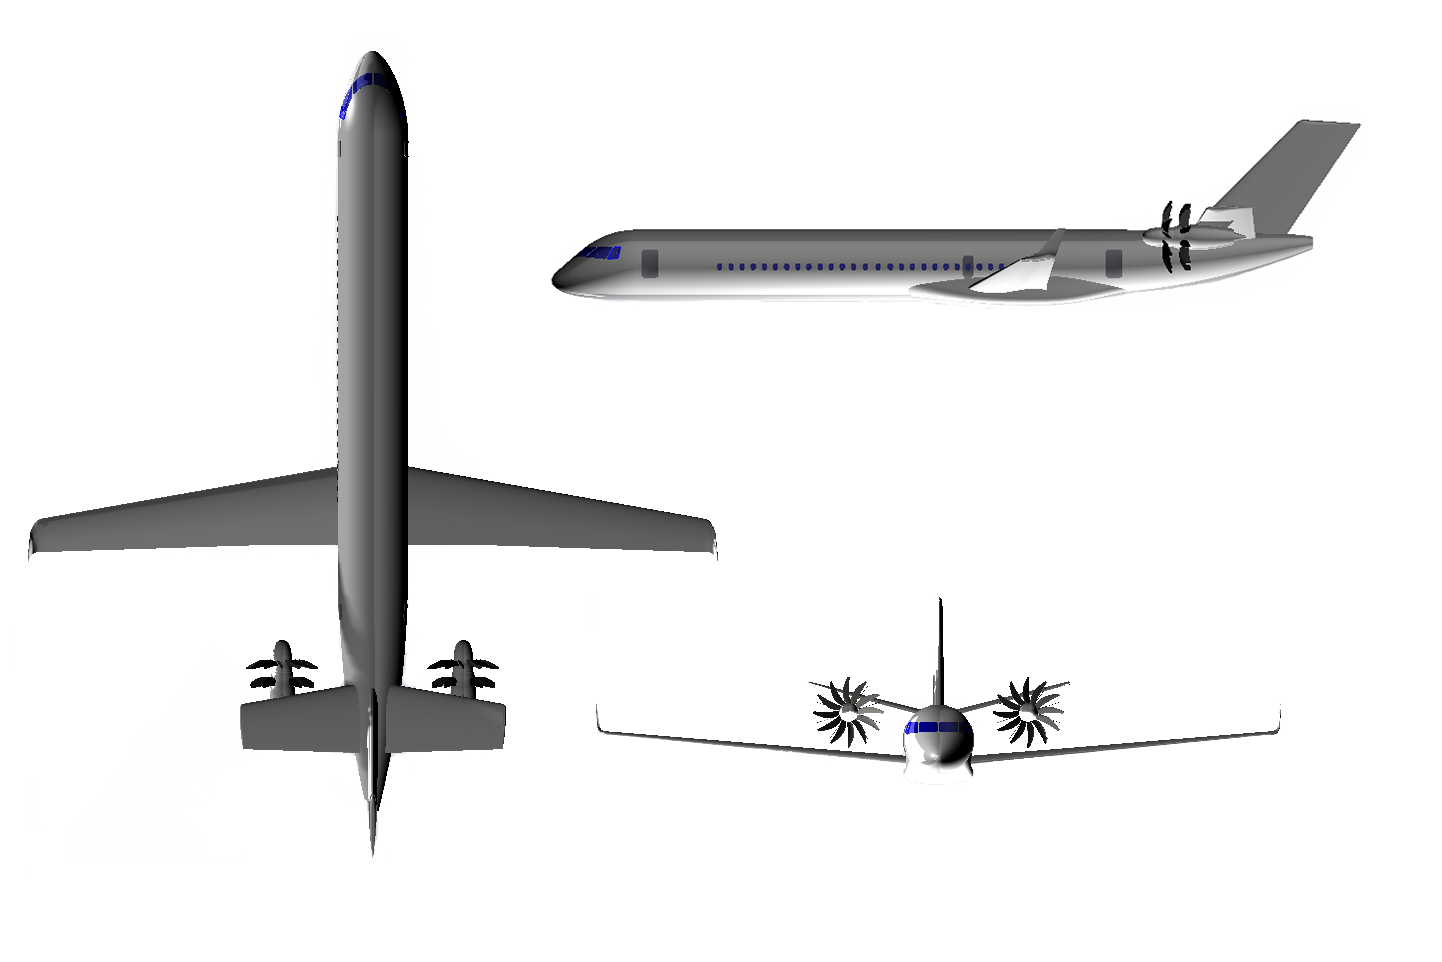
\includegraphics[height=10.5cm, keepaspectratio ]{Immagini/Capitolo3/IRON} 
	\caption{Layout of Regional Turboprop. Side, top and front section.} % didascalia
	\label{fig:figura3_0} % etichetta per citarla nel testo
\end{figure}

\begin{figure}[H]
	\centering
	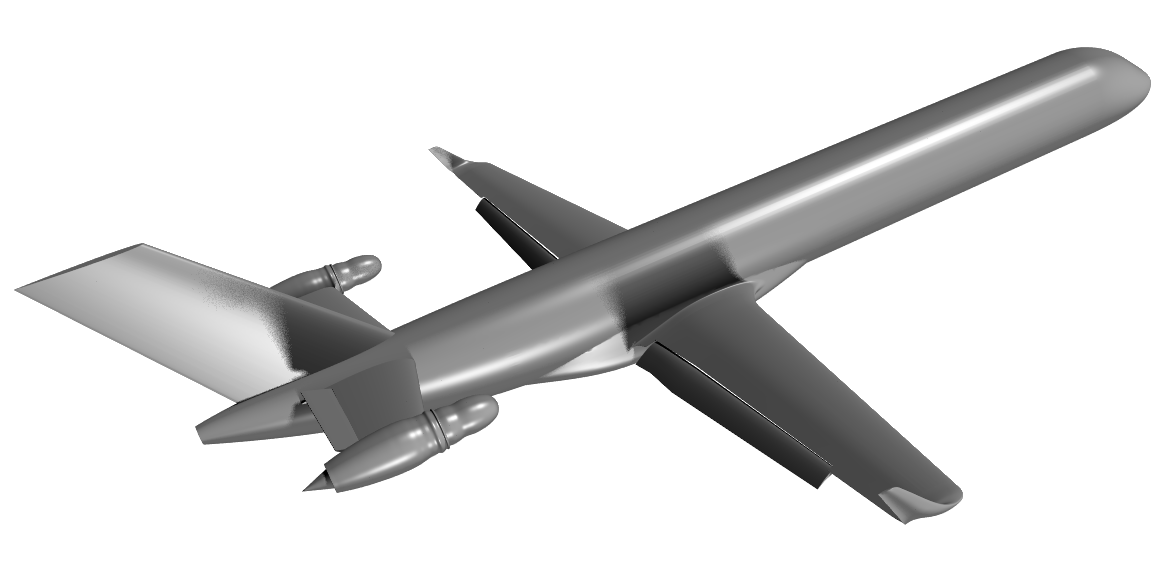
\includegraphics[height=7cm, keepaspectratio ]{Immagini/Capitolo3/IRON_TAKE_OFF} 
	\caption{Regional Turboprop rendering in takeoff configuration} % didascalia
	\label{fig:figura3_01} % etichetta per citarla nel testo
\end{figure}

\begin{table}[H]
\begin{centering}
\begin{tabular}{llc}
\toprule
\textbf{Data}&\textbf{Value} \\
\hline
\multirow{ 7}{*}{Wing}&Span	&	35.34 m	\\
& AR & 12 \\
& $C_r$ & 5.325 m \\
& $C_k$ & 4.5 m \\
& $C_t$ & 3.4 m \\
&  MAC & 3.16 m \\
& Flap type & FOWLER \\
& $\delta_{f_{TO}}$ & $\ang{25}$ \\
\hline
\multirow{4}{*}{Horizontal Tail }&Span	&	12.5 m	\\
& $C_r$ & 3.64 m \\
& $C_t$ & 2.272 m \\
& $\delta_{e_{min}}$ & $\ang{-25}$ \\
\hline
Other data&MTOW	&	51847 kg	\\
\bottomrule

\end{tabular}
\caption{Aircraft main data.}
\label{tabellaB.1}
\end{centering}
\end{table}


\begin{figure}[H]
	%\centering
	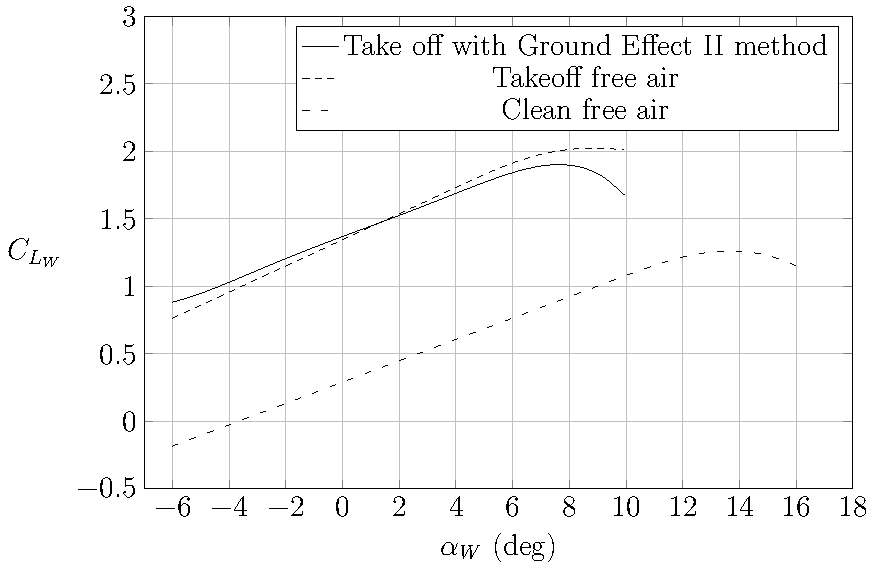
\includegraphics[height=9.5cm, keepaspectratio ]{Immagini/Capitolo3/3_1-GroundEffectOnWingLiftCurve} 
	\caption{Ground effect on wing lift curve} % didascalia
	\label{fig:figura3_1} % etichetta per citarla nel testo
\end{figure}

\begin{figure}[H]
	%\centering
	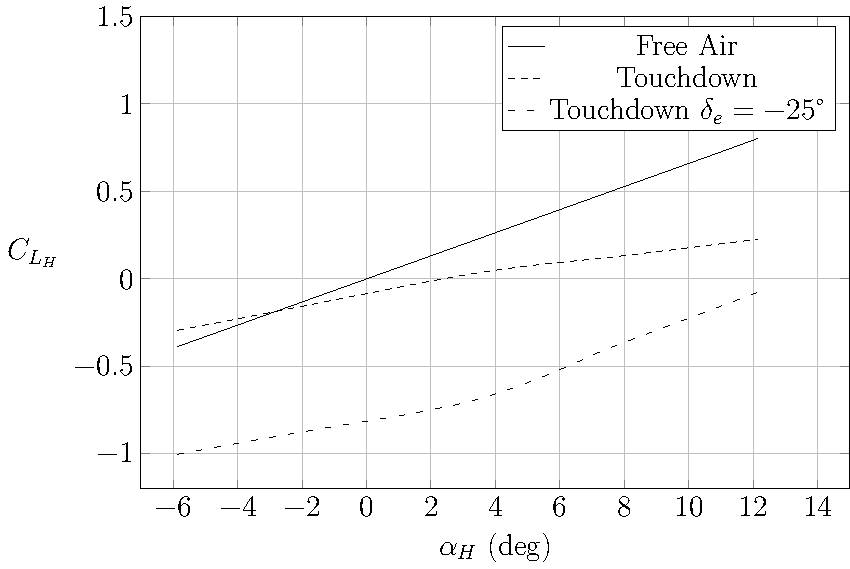
\includegraphics[height=9.5cm, keepaspectratio ]{Immagini/Capitolo3/3_2-GroundEffectOnHorizontalTailLiftCurve} 
	\caption{Ground effect on horizontal tail lift curve} % didascalia
	\label{fig:figura3_2} % etichetta per citarla nel testo
\end{figure}

\begin{figure}[H]
	%\centering
	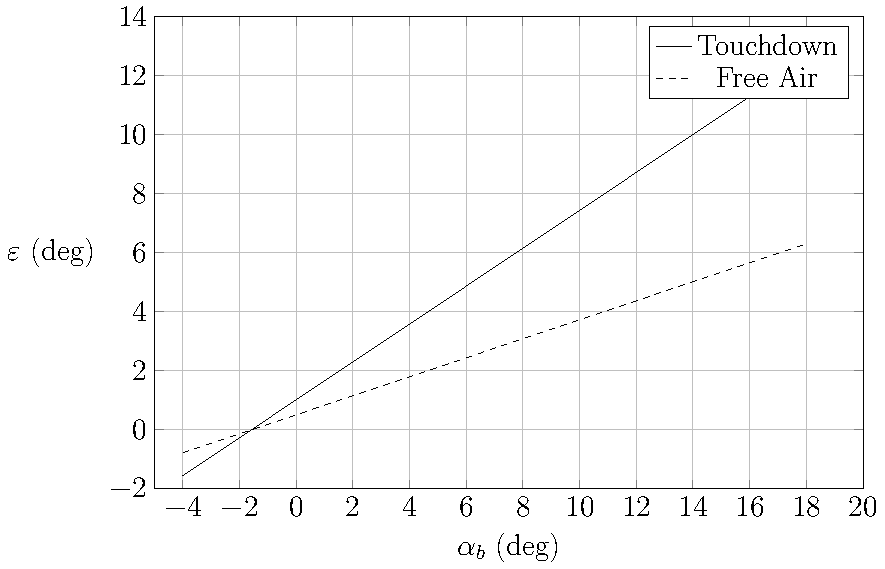
\includegraphics[height=9cm, keepaspectratio ]{Immagini/Capitolo3/3_3-GroundEffectOnDownwashAngle} 
	\caption{Ground effect on downwash angle} % didascalia
	\label{fig:figura3_3} % etichetta per citarla nel testo
\end{figure}

\begin{figure}[H]
	%\centering
	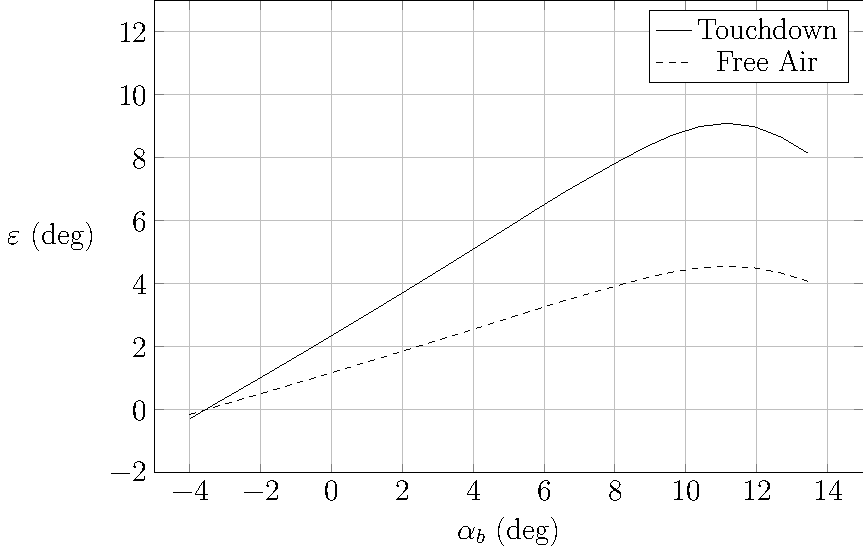
\includegraphics[height=9cm, keepaspectratio ]{Immagini/Capitolo3/3_4-GroundEffectOnDownwashAngleConsideringNonLinearEffects} 
	\caption{Ground effect on downwash angle considering non linear effects} % didascalia
	\label{fig:figura3_4} % etichetta per citarla nel testo
\end{figure}